\documentclass[11pt, a4paper]{article}

\usepackage[margin=1in]{geometry} % Set margins.
\usepackage{enumitem} % Customize lists.
\usepackage{hyperref} % For hyperlinks.
\usepackage{titlesec} % Custom section titles.
\usepackage{graphicx} % Required for including images
\usepackage{float} % For precise placement of the figure
\usepackage{fontawesome} % For icons
\usepackage{adjustbox}
\usepackage{tikz}


% Set section title formatting
\titleformat{\section}
{\large\bfseries} % Format
{} % Label
{0em} % Sep
{} % Before-code
[\titlerule] % After-code

\pagestyle{empty} % No page numbers

\begin{document}
\noindent
\begin{minipage}{0.25\textwidth}
    \begin{tikzpicture}
        \clip (-0.1,0.7) circle (1.9cm); % Adjust the radius as needed
        \node at (0,0) {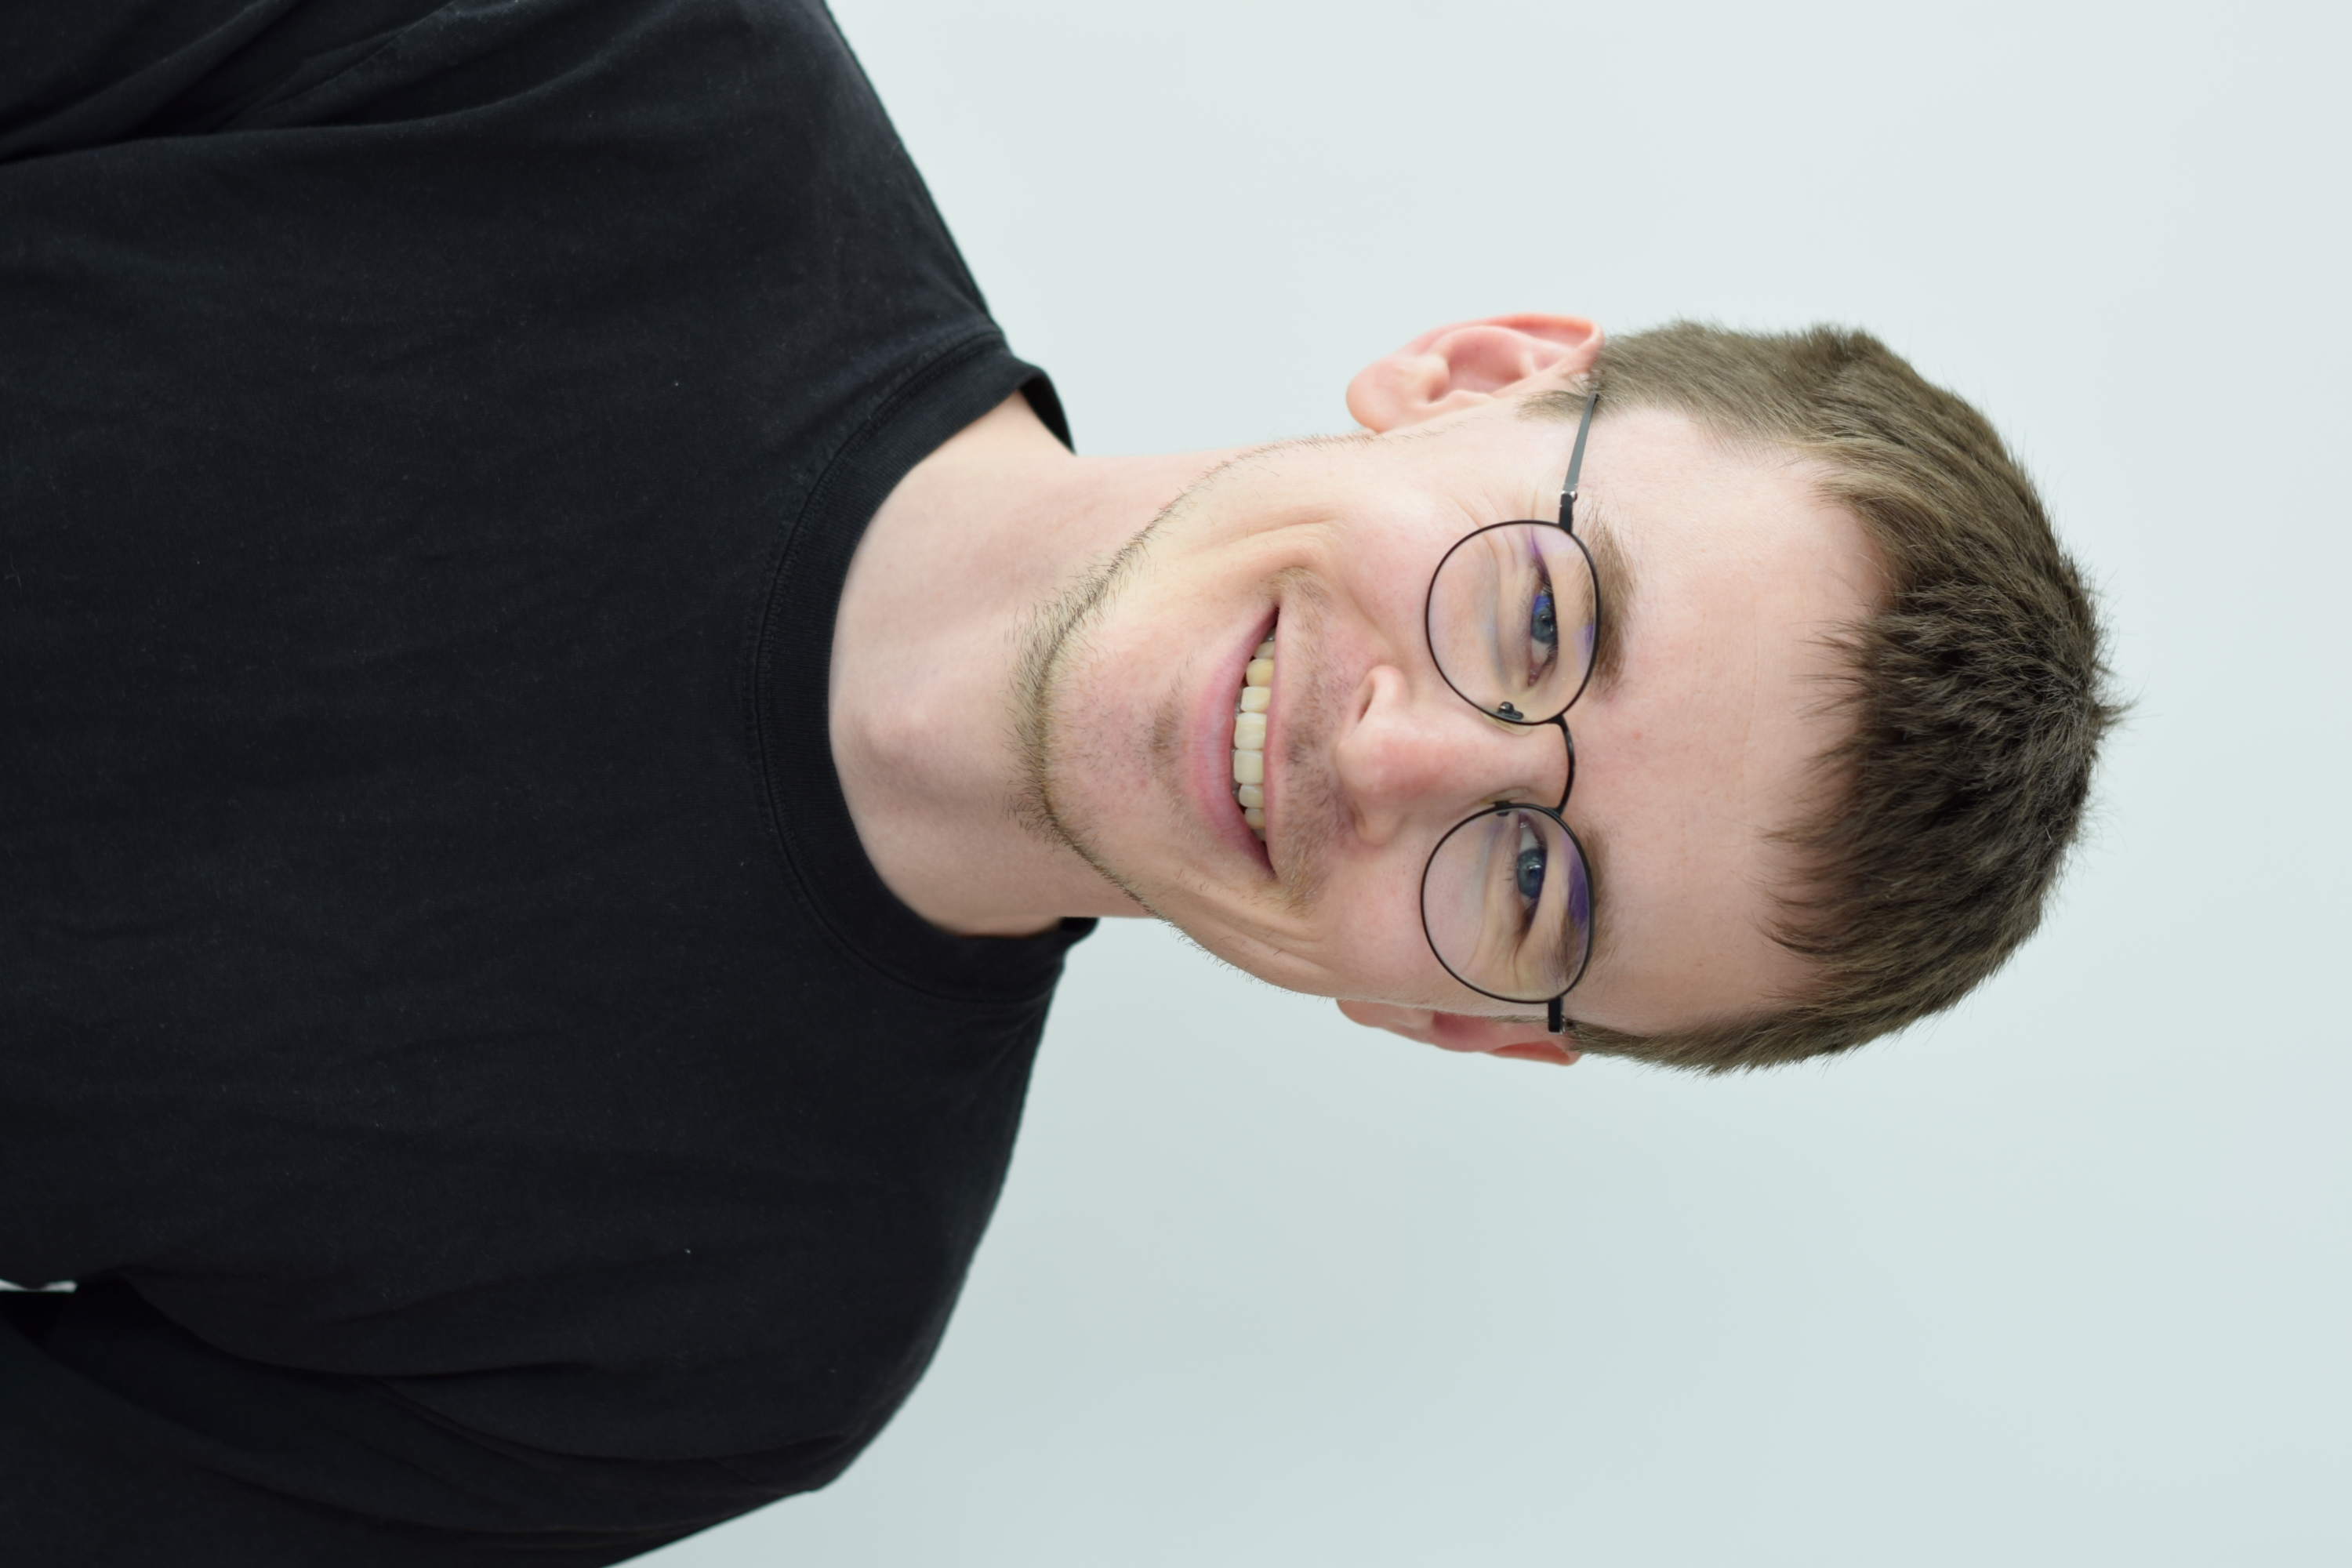
\includegraphics[height=4cm,angle=90]{./assets/profile_pic.jpg}};
    \end{tikzpicture}
\end{minipage}%
\begin{minipage}{0.75\textwidth}
    \centerline{
        \Large\bfseries Frej Sundqvist
    }
    \vspace{0.2em}
    \centerline{
        \textit{Problem solver, Programmer, Engineer}
    }
    \vspace{0.5em}
    \centerline{
        {\faEnvelopeO} \href{mailto:frejsundqvist@protonmail.com}{frejsundqvist@protonmail.com}
        |
        {\faGithub} \href{https://github.com/MyosQ}{MyosQ}
    }
    \centerline{
        {\faLinkedin} \href{https://www.linkedin.com/in/frej-sundqvist-b8a49a14b}{frej-sundqvist-b8a49a14b}
        |
        {\faGlobe} \href{https://www.myosq.github.io/cv}{myosq.github.io/cv}    
    }
\end{minipage}

\vspace{1em}

\section*{Education}
\textbf{University Name}, Degree, \textit{Graduation Year}
\begin{itemize}[noitemsep]
    \item Major: Your Major Here
    \item Relevant coursework: Course 1, Course 2, Course 3
\end{itemize}

\section*{Experience}
\textbf{Job Title}, \textit{Company Name}, Location \hfill Month Year – Present
\begin{itemize}[noitemsep]
    \item Bullet point describing your responsibilities, achievements, technologies used, or projects.
    \item Another bullet point.
\end{itemize}

\textbf{Job Title}, \textit{Company Name}, Location \hfill Month Year – Month Year
\begin{itemize}[noitemsep]
    \item Description.
\end{itemize}

\section*{Projects}
\textbf{Project Title}
\begin{itemize}[noitemsep]
    \item Brief description of your project, technologies used, and your contribution.
    \item GitHub: \href{https://github.com/linktoproject}{linktoproject}
\end{itemize}

\textbf{Project Title}
\begin{itemize}[noitemsep]
    \item Brief description.
\end{itemize}

\section*{Skills}
\begin{itemize}[noitemsep]
    \item Programming Languages: Python, Java, C++
    \item Frameworks/Technologies: Django, React, Docker
    \item Tools: Git, LaTeX, Jenkins
\end{itemize}

\end{document}


% Your other sections follow here...

\end{document}